\documentclass[11pt]{article}
\usepackage{a4}
\usepackage[top=2cm, bottom=2cm, left=2.5cm,  right=2.5cm]{geometry}
\usepackage[pdftex]{graphicx}
\usepackage{latexsym}
\usepackage{multirow}
\usepackage{hyperref}
\usepackage{latexsym}

\usepackage[utf8]{inputenc}
\usepackage{color}
\usepackage{listings}
\definecolor{darkblue}{rgb}{0,0,.5}
\definecolor{lightblue}{rgb}{0,0,1}
\usepackage{tikz}

\renewcommand{\paragraph}[1]{\textbf{#1.}}
%\newcommand{\ignore}[1]{}
\newcommand{\link}[1]{\url{#1}}
\newcommand{\extlink}[1]{\href{#1}{\textbf{$~\triangleright$}}}
\newcommand{\todo}[1]{{\color{red}TODO:#1}}
\newcommand{\comment}[1]{{\color{blue}#1}}
\newcommand{\versailles}[1]{}
\newcommand{\lip}[1]{}

\title{\vspace{0cm}  Report for Data Integration by Ayman YACHAOUI }
\date{}

\newcounter{exercise}
\newcommand{\createExercise}{
\stepcounter{exercise}
\textbf{{\\ Exercise \arabic{exercise}.}}
}

\lstdefinelanguage{XML}
{
  basicstyle=\ttfamily\scriptsize,
  breaklines=true,
  breakatwhitespace=true,
  tabsize=1,
  morestring=[b]",
  moredelim=[s][\bfseries\color{darkblue}]{<}{\ },
  moredelim=[s][\bfseries\color{darkblue}]{</}{>},
  moredelim=[l][\bfseries\color{darkblue}]{/>},
  moredelim=[l][\bfseries\color{darkblue}]{>},
  morecomment=[s]{<!--}{-->},
  morecomment=[s]{<?}{?>},
  morecomment=[s]{<!--}{-->},
  commentstyle=\color{cyan},
  stringstyle=\color{blue},
  identifierstyle=\color{red}
}

\lstdefinelanguage{Java}
{
  language=C,
  basicstyle=\ttfamily\scriptsize,
  breaklines=true,
  breakatwhitespace=true,
  tabsize=1,
  morestring=[b]",
  moredelim=[s][\bfseries\color{darkblue}]{<}{\ },
  moredelim=[s][\bfseries\color{darkblue}]{</}{>},
  moredelim=[l][\bfseries\color{darkblue}]{/>},
  moredelim=[l][\bfseries\color{darkblue}]{>},
  morecomment=[s]{<!--}{-->},
  morecomment=[s]{<?}{?>},
  morecomment=[s]{<!--}{-->},
  commentstyle=\color{grey},
  stringstyle=\color{cyan},
  identifierstyle=\color{darkblue}
}

\newenvironment{myenv}[1]
  {\mdfsetup{
    frametitle={{\tiny \colorbox{white}{\space#1\space}}},
    innertopmargin=0pt,
    frametitleaboveskip=-\ht\strutbox,
    frametitlealignment=\center
    }
  \begin{mdframed}%
  }
  {\end{mdframed}}

\begin{document}
\newtheorem{lemma}{Lemma}
\newtheorem{theorem}{Theorem}
\newtheorem{cor}{Corollary}
\newtheorem{prop}{Proposition}
\newtheorem{Definition}{Definition}
\newtheorem{Proof}{Proof}
\newtheorem{property}{Property}
\newtheorem{subproblem}{Sub-Problem}
\newtheorem{examp}{Example}
%\newtheorem{algorithm}{Algorithm}
\newtheorem{Rule}{Rule}
\newtheorem{condition}{Condition}


\newcommand{\Hybrid}[1]{{\small{\textsf{Hybrid}}}}
\newcommand{\ANGIE}[1]{{\small{\textsf{ANGIE}}}}
\newcommand{\THOMAS}[1]{{\small{\textsf{RDF-3X}}}}
\newcommand{\YAGO}[1]{{\small{\textsf{YAGO}}}}


\newcommand{\blind}[1]{}

\newcommand{\Ex}{{\em \textbf{Example. }}}
\newcommand{\s}[1]{{\small{\textsf{#1}}}}
\newcommand{\SQ}[1]{{\small{\textsf{#1}}}}
\newcommand{\W}[1]{{\em {#1}}}





\newcommand\alkis[1]{{\color{blue} $\parallel$\textbf{Alkis}: #1 $\parallel$}}
\newcommand\serge[1]{{\color{red} $\parallel$\textbf{Serge}: #1 $\parallel$}}
\newcommand\nico[1]{{\color{blue}    #1   }}



\newcommand\calD{\ensuremath{\mathcal D}}
\newcommand\calB{\ensuremath{\mathcal B}}
\newcommand\calP{\ensuremath{\mathcal P}}
\newcommand\calI{\ensuremath{\mathcal I}}
\newcommand\calL{\ensuremath{\mathit{Label}}}
\newcommand{\cut}{\ensuremath{{\it cut}}}
\newcommand\locatepeers{{\tt locateXML}}

%\newcommand\ABF{\ensuremath{BF_{\alpha}}}
\newcommand\ABF{{\it ABF}}
%\newcommand\DBF{\ensuremath{BF_{\delta}}}
\newcommand\DBF{{\it DBF}}
\newcommand\anc{\ensuremath{ \backslash\backslash}}
\newcommand\stitle[1]{{\vpar\noindent{\bf #1}}}

\newcommand\vpar{{\vspace*{0.5em}}}

\newcommand{\csbbox}{\vrule height7pt width4pt depth1pt}

\newcommand{\fp}{\mathit{fp}}

\newtheorem{defn}{Definition}[section]
\newtheorem{thm}{Theorem}[section]
\newtheorem{lem}{Lemma}[section]

\newtheorem{CSEXAMPLE}{Example}[section]
\newenvironment{csexample}{\begin{CSEXAMPLE} \hspace{-.85em} {\bf :} \rm}%
                            {\end{CSEXAMPLE}}

\newenvironment{remark}{\stitle{Remark.}}{}

\newcommand{\csxam}{\begin{csexample}}
\newcommand{\csexam}{\csbbox\end{csexample}}

\newcommand{\csprf}{\noindent{\bf Proof:}}
\newcommand{\cseprf}{\csbbox}

\newcounter{ccc}
\newcommand{\bcc}{\setcounter{ccc}{1}\theccc.}
\newcommand{\icc}{\addtocounter{ccc}{1}\theccc.}

\newcommand\utitle[1]{{\vpar\noindent{\underline{#1}}}}
\newcommand\sutitle[1]{{\vpar\noindent{\textbf{\underline{#1}}}}}
\newcommand\bstitle[1]{{\noindent{\bf #1}}}

\newcommand\queryplan[3][@R=8pt @C=2pt]{{\small \begin{minipage}[th]{#2}\xymatrix
    #1 {#3}\end{minipage}}}
\newcommand\querytree\queryplan

\newcommand\notes[1]{{\bf $\|$~{#1}~$\|$}}

\newcommand\given{\ensuremath{~|~}}

\newcommand\eat[1]{}

\newcommand\minarg{\ensuremath{\operatornamewithlimits{minarg}}}
\newenvironment{pseudocode}{\begin{tabbing}llllll\=llll\=llll\=llll\=llll\=llll\kill\small}{\end{tabbing}}

\newcommand{\myhrule}{\rule[.5pt]{\hsize}{.5pt}}
\newcommand\smalltt[1]{\textsf{\small{#1}}}
%% Section spacing
%\newcommand{\oespace}{\vspace*{-1.8em}}
%\newcommand{\osspace}{\vspace*{-1.6em}}
%\newcommand{\ofspace}{\vspace*{-1.4em}}
%\newcommand{\otspace}{\vspace*{-1.2em}}
%\newcommand{\ospace}{\vspace*{-1em}}
%\newcommand{\espace}{\vspace*{-2mm}}
%\newcommand{\sspace}{\vspace*{-.6em}}
%\newcommand{\fspace}{\vspace*{-.4em}}
%\newcommand{\tspace}{\vspace*{-.2em}}


\newcommand{\pfspace}{\vspace*{.4em}}
\newcommand{\ptspace}{\vspace*{.2em}}
\newcommand{\paraspace}{\pfspace}

%%%%%%%%%%%% Fabian's macros

%\renewcommand{\algorithmicrequire}{\textbf{Input:}}
%\renewcommand{\algorithmiccomment}[1]{$~~~~$ //#1}
\newcommand{\ignore}[1]{}
% Fabian: I think we should use a uniform appearance of all entities
% in the text. It has proven useful to treat relations, entities and facts
% alike. Feel free to change the layout as you like it.
\newcommand{\entity}[1]{{\textit{#1}}}
%\newcommand{\var}[1]{{\textit{\$#1}}}
\newcommand{\newWord}[1]{\emph{#1}}

\newcounter{figureCounter}
\newcommand{\ffigure}[4]{% \ffigure[th]{label}{title}{imagecommand}{vskip}
\ \\[-0.0cm]
  \refstepcounter{figureCounter} \label{#1}
  {\centering #3\\[-#4]}
  {\centering \bf Figure \ref{#1}: #2\\[0.2cm]}
}
\newcommand{\para}[1]{\noindent{\textbf{#1.}}}


\newcommand{\hls}{{\small $<$}}
\newcommand{\hg}{{\small $>$}}

\pagestyle{empty}

\huge{Report for Data Integration project by Ayman YACHAOUI\\}
\normalsize {}

The program I have written takes an aribitrary number of WS's provided with their definitions and realizes joins based on arbitrary number of variable matching. It is aimed to be as generic as possible and often trades performance for the completeness of the view as will be discussed. What follows is a running example of my implementation and source code comments on its details. To demonstrate its abilities, let's run through this demonstration query:\\
\begin{center}
mb\_getArtistInfoByName("skrillex", ?id, ?b, ?e)\\
					\#mb\_getReleasesByArtistId(?id,?asin,?releaseid,?title,?date)\\
					\#mb\_getReleasesByArtist(?id,?asin, ?title, ?date)\\
					\#mb\_getTrackByReleaseId(?tracktitle,?duration,?trackid,?releaseid)\\
\end{center}
This query is composed of 4 steps:
\begin{enumerate}
\item By entering an artist name, the artist id (?id), her birth date (?b) and death date (?e) are returned.
\item The (?id) variables are cascaded down to get the albums produced by the artist. The album ASIN number (?asin), the album id (?releaseid), the album title (?title) and date of release (?date) are output.
\item The third step is redundant and used to demonstrate ability to match several variables from preceding outputs and returns the same data as for the 2nd step.
\item Using the album id (?releaseid), the 4th step outputs all the songs within it with their titles (?tracktitle), song duration (?duration), a song id (?trackid).
\end{enumerate}
\section{WS definitions}
The .xsl definitions schema is unaltered when each .xml definition is articulated in 4 sections.
\begin{itemize}
\item \begin{lstlisting}[language=XML]
<headvariables/> , <call/> and <transformation/>
\end{lstlisting}
as defined and used by Pr Preda
\item \begin{lstlisting}[language=XML]
<partialmerge/>
\end{lstlisting}
used in the merging of XML subcalls as discussed in section.\\
\end{itemize}
As an illustration, here's the definition for mb\_getReleasesByArtist:
\begin{lstlisting}[language=XML]
<?xml version="1.0" encoding="UTF-8" standalone="yes"?>
<ws>

	<prefix name="w" value="http://www.w3.org/1999/02/22-rdf-syntax-ns#"/>
	<prefix name="y" value="http://mpii.de/yago/resource/"/>
	
	<headVariables>
        <variable type="inout" name="?artistid"/>
        <variable type="inout" name="?asin"/>
        <variable type="inout" name="?title"/>
        <variable type="output" name="?type"/>
        <variable type="output" name="?date"/>
    </headVariables>
    
	<definition>
	</definition>
	
	<call>
		<part type="constant" value="http://musicbrainz.org/ws/1/release/?artistid="/>
		<part type="input" variable="?artistid" class="singer" separator="+" />
		<part type="constant" value="?asin="/>
		<part type="input" variable="?asin" class="uk" separator="+" />
		<part type="constant" value="?title="/>
		<part type="input" variable="?title" class="uk2" separator="+" />
	</call>
	
	<transformation file="mb_getReleasesByArtistId.xsl"/>
	
	<partialmerge container_tags="metadata,release-list"/>

</ws>
\end{lstlisting}
\section{Query plan}
\subsection{Class variables}
The main static structures maintained throught the engine processing of a query are :
\begin{center}
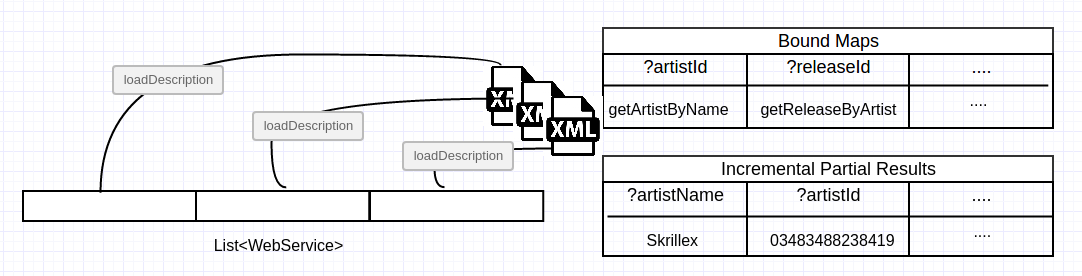
\includegraphics[width=\linewidth]{static.png}
\end{center}
\begin{itemize}
\item An \textbf{Array} of web services is filled using the \textit{loadDescription} method using the .xml descriptions.
\item For every webservice varible, an entry is created in the \textbf{BoundMaps} TreeMap which references the WS needed for an eventual join.
\item At the end of each step of the query, an ArrayList of String[ ] \textbf{incrementalPartialResults} is created storing the result rows that match the current step so far in the query.
\end{itemize}
\subsection{Execution flow}
\subsubsection{Getting the data}
For each step, we call the WS with the appropriate URLs, the following chart sums up this process:
\begin{center}
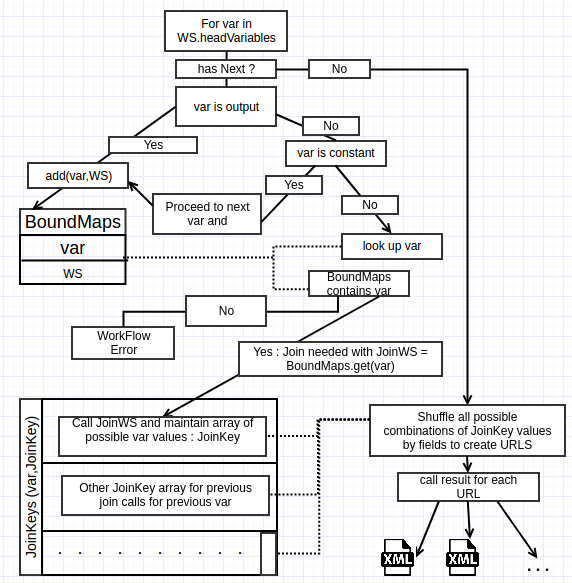
\includegraphics[height=0.38\paperheight]{DataGetterFlowChart.png}
\end{center}
It is worth noting that in the case of joining several columns for a single WS, the URLs are generated so as to cover every possible combination of needed field values. One could note that this dramatically slows down the data getting phase since it's going to collect mostly empty call results but this ensures that \textbf{join columns are independent}. And can even come from different API's !
\subsubsection{Joining the data}
We then proceed to filling \textbf{incrementalPartialResults}. This is done iteratively at the end of \textit{Getting the data} phase of each WS. We distinguish 2 starting points:
\begin{itemize}
\item The WS calls resulted in several XML partial calls, we merge them into a single one, which brings us to the second starting point.
\item The WS call resulted in a single xml of call result, we transform it using \textit{getTransformationResult}
\end{itemize}
The transformed file is \textbf{listOfTupleResults} that is used to join \textbf{incrementalPartialResults}. For every row1 in \textbf{incrementalPartialResults}, its fields are compared to every row2 in \textbf{listOfTupleResults}, if they match, row2 is appended to row1 and maintained in a newer version (thus incremental) PartialResults.
\section{Running example}
We comment here some of the console output that tracks the execution of the query plan:\\
The first webservice \textbf{GetArtistByName} results in a single .xml call result.
\begin{center}
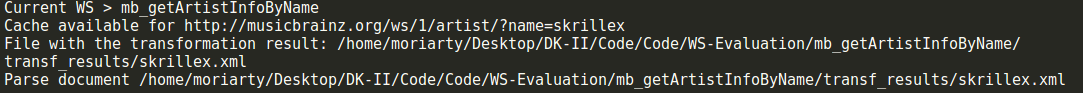
\includegraphics[width=\linewidth]{ws1.png}
\end{center}
After the result of the first webservice are joined with the (intially empty thus appended) \textbf{incrementalPartialResults}, The second webservice \textbf{GetReleaseByArtistId} is called. It needs the \textit{?artistid} field which it gets from calling the transformed result from WS1. Two artist go by that name and thus spawn two URL calls. These will be merged than transformed and be a basis if WS2 is called for its results later before being joined to the existing \textbf{incrementalPartialResults}, maintaining only valid rows:
\begin{center}
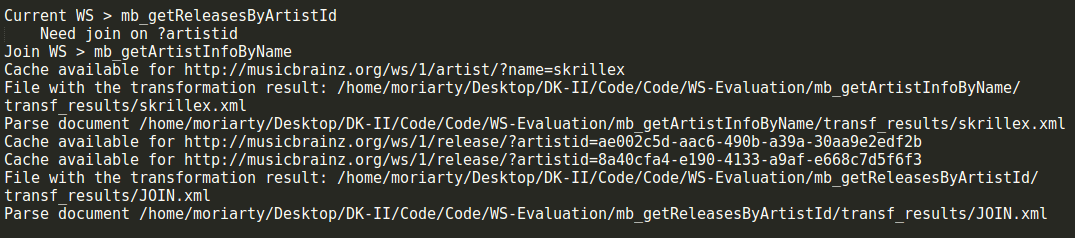
\includegraphics[width=\linewidth]{ws2.png}
\end{center}
The third web-service \textbf{GetReleaseByArtist} outputs the same data as WS2 and is used here to demonstrate the join key shuffling that occurs. Indeed \textbf{GetReleaseByArtistId} needs as input the \textit{?asin} and \textit{?title} which it gets from WS2 for which they are rather defined as outputs.
\begin{center}
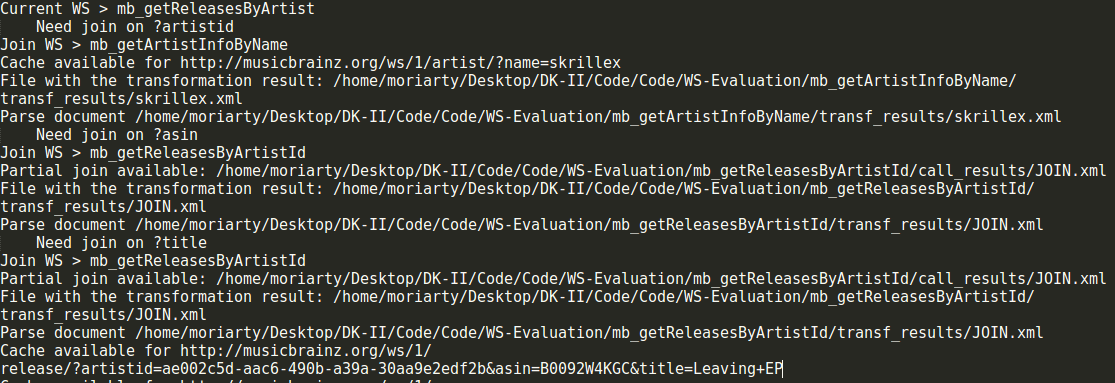
\includegraphics[width=\linewidth]{ws3.png}
\end{center}
This process can go on indefinitely for an arbitrary number of WS's. After the 4th and last WS is processed, the results (which are stored in \textbf{incrementalPartialResults}) are printed in tabular form.
\bibliographystyle{plain}
\bibliography{bib}
\end{document}


